\documentclass{beamer}
\usetheme{Berkeley}
\usecolortheme{seahorse}
\usepackage[brazil]{babel}
\usepackage[utf8]{inputenc}
\usepackage[T1]{fontenc}
\usepackage{lmodern}

\title{G-RAM \& VG-RAM}
\author{Bruno Lima \and Daniel Alves}
\date{}

\setbeamercolor{alerted text}{fg = green}

\begin{document}
\titlepage

\begin{frame}
    \frametitle{Sumário}
    \tableofcontents
%    \begin{itemize}
        %\item Background 
        %\item GRAM
		%\begin{itemize}
			%\item Motivação
			%\item Propagação
			%\item Exemplo
		%\end{itemize}
        %\item VG-RAM
		%\begin{itemize}
			%\item Motivação
			%\item Estratégia
			%\item Células de Minchinton
			%\item Exemplo
		%\end{itemize}
		%\item Bibliografia
%    \end{itemize}
\end{frame}
\section{Background}
\begin{frame}
    \frametitle{Background}
    \begin{itemize}
        \item tipo de neurônio
        \item seguem PLN - estado $u$
        \item propagação
    \end{itemize}
\end{frame}
\section{G-RAM}
\subsection{Motivação}
\begin{frame}
    \frametitle{G-RAM}
    \begin{itemize}
        \item tipo de neurônio
        \item seguem PLN - estado $u$
        \item treino pequeno: hesitação
        \item diferencial: propagação
    \end{itemize}
\end{frame}
\subsection{Propagação}
\begin{frame}
    \frametitle{Propagação}
    \begin{itemize}
        \item atribuição no endereço
        \item propagação até distância máxima $d$
        \item distância de Hamming; exemplo:
            \begin{itemize}
                \item 10\alert 0101 e 10\alert 1101: 1
                \item \alert 10\alert 010\alert 1 e \alert 00\alert 110\alert 0: 3
            \end{itemize}
        \item resultado: núcleos de padrões
    \end{itemize}
\end{frame}
\subsection{Exemplo}
\begin{frame}
    \frametitle{Exemplo da G-RAM}
    G-RAM com 6 bits e $d = 2$. Valores iniciais:

    \begin{table}
        \centering
        \begin{tabular}{|c|c|c|c|c|c|c|c|c|}
            \hline
                & 000 & 001 & 010 & 011 & 100 & 101 & 110 & 111\\
            \hline
            000 &  u  &  u  &  u  &  u  &  u  &  u  &  u  &  u \\
            \hline
            001 &  u  &  u  &  u  &  u  &  u  &  u  &  u  &  u \\
            \hline
            010 &  u  &  u  &  u  &  u  &  u  &  u  &  u  &  u \\
            \hline
            011 &  u  &  u  &  u  &  u  &  u  &  u  &  u  &  u \\
            \hline
            100 &  u  &  u  &  u  &  u  &  u  &  u  &  u  &  u \\
            \hline
            101 &  u  &  u  &  u  &  u  &  u  &  u  &  u  &  u \\
            \hline
            110 &  u  &  u  &  u  &  u  &  u  &  u  &  u  &  u \\
            \hline
            111 &  u  &  u  &  u  &  u  &  u  &  u  &  u  &  u \\
            \hline

        \end{tabular}
    \end{table}
\end{frame}
\begin{frame}
    \frametitle{Exemplo da G-RAM}
    Valor de treino 100011 associado a 1:

    \begin{table}
        \centering
        \begin{tabular}{|c|c|c|c|c|c|c|c|c|}
            \hline
                & 000 & 001 & 010 & 011 & 100 & 101 & 110 & 111\\
            \hline
            000 &  u  &  u  &  u  &  u  &  u  &  u  &  u  &  u \\
            \hline
            001 &  u  &  u  &  u  &  u  &  u  &  u  &  u  &  u \\
            \hline
            010 &  u  &  u  &  u  &  u  &  u  &  u  &  u  &  u \\
            \hline
            011 &  u  &  u  &  u  &  u  &  \alert 1  &  u  &  u  &  u \\
            \hline
            100 &  u  &  u  &  u  &  u  &  u  &  u  &  u  &  u \\
            \hline
            101 &  u  &  u  &  u  &  u  &  u  &  u  &  u  &  u \\
            \hline
            110 &  u  &  u  &  u  &  u  &  u  &  u  &  u  &  u \\
            \hline
            111 &  u  &  u  &  u  &  u  &  u  &  u  &  u  &  u \\
            \hline

        \end{tabular}
    \end{table}
\end{frame}
\begin{frame}
    \frametitle{Exemplo da G-RAM}
    Propagação para distância 1:

    \begin{table}
        \centering
        \begin{tabular}{|c|c|c|c|c|c|c|c|c|}
            \hline
                & 000 & 001 & 010 & 011 & 100 & 101 & 110 & 111\\
            \hline
            000 &  u  &  u  &  u  &  u  &  u  &  u  &  u  &  u \\
            \hline
            001 &  u  &  u  &  u  &  u  &  \alert 1  &  u  &  u  &  u \\
            \hline
            010 &  u  &  u  &  u  &  u  &  \alert 1  &  u  &  u  &  u \\
            \hline
            011 &  \alert 1  &  u  &  u  &  u  &  1  &  \alert 1  &  \alert 1  &  u \\
            \hline
            100 &  u  &  u  &  u  &  u  &  u  &  u  &  u  &  u \\
            \hline
            101 &  u  &  u  &  u  &  u  &  u  &  u  &  u  &  u \\
            \hline
            110 &  u  &  u  &  u  &  u  &  u  &  u  &  u  &  u \\
            \hline
            111 &  u  &  u  &  u  &  u  &  \alert 1  &  u  &  u  &  u \\
            \hline

        \end{tabular}
    \end{table}
\end{frame}
\begin{frame}
    \frametitle{Exemplo da G-RAM}
    Propagação para distância 2:

    \begin{table}
        \centering
        \begin{tabular}{|c|c|c|c|c|c|c|c|c|}
            \hline
                &       000 &       001 &       010 &       011 &       100 &       101 &       110 &       111\\
            \hline
            000 &        u  &        u  &        u  &        u  & \alert 1  &        u  &        u  &        u \\
            \hline
            001 & \alert 1  &        u  &        u  &        u  &        1  & \alert 1  & \alert 1  &        u \\
            \hline
            010 & \alert 1  &        u  &        u  &        u  &        1  & \alert 1  & \alert 1  &        u \\
            \hline
            011 &        1  & \alert 1  & \alert 1  &        u  &        1  &        1  &        1  & \alert 1 \\
            \hline
            100 &        u  &        u  &        u  &        u  &        1  &        u  &        u  &        u \\
            \hline
            101 &        u  &        u  &        u  &        u  & \alert 1  &        u  &        u  &        u \\
            \hline
            110 &        u  &        u  &        u  &        u  & \alert 1  &        u  &        u  &        u \\
            \hline
            111 & \alert 1  &        u  &        u  &        u  &        1  & \alert 1  & \alert 1  &        u \\
            \hline

        \end{tabular}
    \end{table}
\end{frame}
\begin{frame}
    \frametitle{Exemplo da G-RAM}
    Valor de treino 011100 associado a 1:

    \begin{table}
        \centering
        \begin{tabular}{|c|c|c|c|c|c|c|c|c|}
            \hline
                &       000 &       001 &       010 &       011 &       100 &       101 &       110 &       111\\
            \hline
            000 &        u  &        u  &        u  &        u  &        1  &        u  &        u  &        u \\
            \hline
            001 &        1  &        u  &        u  &        u  &        1  &        1  &        1  &        u \\
            \hline
            010 &        1  &        u  &        u  &        u  &        1  &        1  &        1  &        u \\
            \hline
            011 &        1  &        1  &        1  &        u  &        1  &        1  &        1  &        1 \\
            \hline
            100 &        u  &        u  &        u  & \alert 1  &        1  &        u  &        u  &        u \\
            \hline
            101 &        u  &        u  &        u  &        u  &        1  &        u  &        u  &        u \\
            \hline
            110 &        u  &        u  &        u  &        u  &        1  &        u  &        u  &        u \\
            \hline
            111 &        1  &        u  &        u  &        u  &        1  &        1  &        1  &        u \\
            \hline

        \end{tabular}
    \end{table}
\end{frame}
\begin{frame}
    \frametitle{Exemplo da G-RAM}
    Propagação para distância 1:

    \begin{table}
        \centering
        \begin{tabular}{|c|c|c|c|c|c|c|c|c|}
            \hline
                &       000 &       001 &       010 &       011 &       100 &       101 &       110 &       111\\
            \hline
            000 &        u  &        u  &        u  & \alert 1  &        1  &        u  &        u  &        u \\
            \hline
            001 &        1  &        u  &        u  &        u  &        1  &        1  &        1  &        u \\
            \hline
            010 &        1  &        u  &        u  &        u  &        1  &        1  &        1  &        u \\
            \hline
            011 &        1  &        1  &        1  &        u  &        1  &        1  &        1  &        1 \\
            \hline
            100 &        u  & \alert 1  & \alert 1  &        1  &        1  &        u  &        u  & \alert 1 \\
            \hline
            101 &        u  &        u  &        u  & \alert 1  &        1  &        u  &        u  &        u \\
            \hline
            110 &        u  &        u  &        u  & \alert 1  &        1  &        u  &        u  &        u \\
            \hline
            111 &        1  &        u  &        u  &        u  &        1  &        1  &        1  &        u \\
            \hline

        \end{tabular}
    \end{table}
\end{frame}
\begin{frame}
    \frametitle{Exemplo da G-RAM}
    Propagação para distância 2:

    \begin{table}
        \centering
        \begin{tabular}{|c|c|c|c|c|c|c|c|c|}
            \hline
                &       000 &       001 &       010 &       011 &       100 &       101 &       110 &       111\\
            \hline
            000 &        u  & \alert 1  & \alert 1  &        1  &        1  &        u  &        u  & \alert 1 \\
            \hline
            001 &        1  &        u  &        u  & \alert 1  &        1  &        1  &        1  &        u \\
            \hline
            010 &        1  &        u  &        u  & \alert 1  &        1  &        1  &        1  &        u \\
            \hline
            011 &        1  &        1  &        1  &        u  &        1  &        1  &        1  &        1 \\
            \hline
            100 & \alert 1  &        1  &        1  &        1  &        1  & \alert 1  & \alert 1  &        1 \\
            \hline
            101 &        u  & \alert 1  & \alert 1  &        1  &        1  &        u  &        u  & \alert 1 \\
            \hline
            110 &        u  & \alert 1  & \alert 1  &        1  &        1  &        u  &        u  & \alert 1 \\
            \hline
            111 &        1  &        u  &        u  & \alert 1  &        1  &        1  &        1  &        u \\
            \hline

        \end{tabular}
    \end{table}
\end{frame}
\begin{frame}
    \frametitle{Exemplo da G-RAM}
    Valor de treino 001111 associado a 0:

    \begin{table}
        \centering
        \begin{tabular}{|c|c|c|c|c|c|c|c|c|}
            \hline
                &       000 &       001 &       010 &       011 &       100 &       101 &       110 &       111\\
            \hline
            000 &        u  &        1  &        1  &        1  &        1  &        u  &        u  &        1 \\
            \hline
            001 &        1  &        u  &        u  &        1  &        1  &        1  &        1  &        u \\
            \hline
            010 &        1  &        u  &        u  &        1  &        1  &        1  &        1  &        u \\
            \hline
            011 &        1  &        1  &        1  &        u  &        1  &        1  &        1  &        1 \\
            \hline
            100 &        1  &        1  &        1  &        1  &        1  &        1  &        1  &        1 \\
            \hline
            101 &        u  &        1  &        1  &        1  &        1  &        u  &        u  &        1 \\
            \hline
            110 &        u  &        1  &        1  &        1  &        1  &        u  &        u  &        1 \\
            \hline
            111 &        1  & \alert 0  &        u  &        1  &        1  &        1  &        1  &        u \\
            \hline

        \end{tabular}
    \end{table}
\end{frame}
\begin{frame}
    \frametitle{Exemplo da G-RAM}
    Propagação para distância 1 - colisões:

    \begin{table}
        \centering
        \begin{tabular}{|c|c|c|c|c|c|c|c|c|}
            \hline
                &       000 &       001 &       010 &       011 &       100 &       101 &       110 &       111\\
            \hline
            000 &        u  &        1  &        1  &        1  &        1  &        u  &        u  &        1 \\
            \hline
            001 &        1  &        u  &        u  &        1  &        1  &        1  &        1  &        u \\
            \hline
            010 &        1  &        u  &        u  &        1  &        1  &        1  &        1  &        u \\
            \hline
            011 &        1  & \alert 0  &        1  &        u  &        1  &        1  &        1  &        1 \\
            \hline
            100 &        1  &        1  &        1  &        1  &        1  &        1  &        1  &        1 \\
            \hline
            101 &        u  & \alert 1  &        1  &        1  &        1  &        u  &        u  &        1 \\
            \hline
            110 &        u  & \alert 1  &        1  &        1  &        1  &        u  &        u  &        1 \\
            \hline
            111 & \alert 0  &        0  &        u  & \alert 1  &        1  & \alert 1  &        1  &        u \\
            \hline

        \end{tabular}
    \end{table}
    Colisões: seleção aleatória ou indefinição
\end{frame}
\begin{frame}
    \frametitle{Exemplo da G-RAM}
    Propagação para distância 2 - colisões:

    \begin{table}
        \centering
        \begin{tabular}{|c|c|c|c|c|c|c|c|c|}
            \hline
                &       000 &       001 &       010 &       011 &       100 &       101 &       110 &       111\\
            \hline
            000 &        u  &        1  &        1  &        1  &        1  &        u  &        u  &        1 \\
            \hline
            001 &        1  & \alert 0  &        u  &        1  &        1  &        1  &        1  &        u \\
            \hline
            010 &        1  & \alert 0  &        u  &        1  &        1  &        1  &        1  &        u \\
            \hline
            011 & \alert 0  &        u  &        1  & \alert 0  &        1  &        1  &        1  &        1 \\
            \hline
            100 &        1  & \alert 0  &        1  &        1  &        1  &        1  &        1  &        1 \\
            \hline
            101 & \alert 0  &        1  &        1  & \alert 0  &        1  & \alert 0  &        u  &        1 \\
            \hline
            110 & \alert 0  &        1  &        1  & \alert 0  &        1  & \alert 0  &        u  &        1 \\
            \hline
            111 &        0  &        0  & \alert 0  &        1  & \alert 0  &        1  &        1  & \alert 0 \\
            \hline

        \end{tabular}
    \end{table}
\end{frame}
\begin{frame}
    \frametitle{Exemplo da G-RAM}
    Consultas:

    \begin{table}
        \centering
        \begin{tabular}{|c|c|c|c|c|c|c|c|c|}
            \hline
                &       000 &       001 &       010 &       011 &       100 &       101 &       110 &       111\\
            \hline
            000 &        u  &        1  &        1  &        1  &        1  &        u  &        u  &        1 \\
            \hline
            001 &        1  &        0  &        u  &        1  &        1  &        1  &        1  &        u \\
            \hline
            010 &        1  &        0  &        u  &        1  &        1  &        1  &        1  &        u \\
            \hline
            011 &        0  &        u  &        1  &        0  &        1  &        1  &        1  &        1 \\
            \hline
            100 &        1  &        0  &        1  &        1  &        1  &        1  &        1  &        1 \\
            \hline
            101 &        0  &        1  &        1  &        0  &        1  &        0  &        u  &        1 \\
            \hline
            110 &        0  &        1  &        1  & \alert 0  &        1  &        0  &        u  &        1 \\
            \hline
            111 &        0  &        0  &        0  &        1  &        0  &        1  &        1  &        0 \\
            \hline

        \end{tabular}
    \end{table}
    \begin{description}
        \item[011110] 0
    \end{description}
\end{frame}
\begin{frame}
    \frametitle{Exemplo da G-RAM}
    Consultas:

    \begin{table}
        \centering
        \begin{tabular}{|c|c|c|c|c|c|c|c|c|}
            \hline
                &       000 &       001 &       010 &       011 &       100 &       101 &       110 &       111\\
            \hline
            000 &        u  &        1  &        1  &        1  &        1  &        u  &        u  &        1 \\
            \hline
            001 &        1  &        0  &        u  &        1  &        1  &        1  &        1  &        u \\
            \hline
            010 &        1  &        0  &        u  &        1  &        1  &        1  &        1  &        u \\
            \hline
            011 &        0  &        u  &        1  &        0  &        1  &        1  &        1  &        1 \\
            \hline
            100 &        1  &        0  &        1  &        1  &        1  &        1  &        1  &        1 \\
            \hline
            101 &        0  &        1  &        1  &        0  &        1  &        0  &        u  &        1 \\
            \hline
            110 &        0  & \alert 1  &        1  &        0  &        1  &        0  &        u  &        1 \\
            \hline
            111 &        0  &        0  &        0  &        1  &        0  &        1  &        1  &        0 \\
            \hline
        \end{tabular}
    \end{table}
    \begin{description}
        \item[001110] 1
    \end{description}
\end{frame}
\section{VG-RAM}
\subsection{Motivação}
\begin{frame}
    \frametitle{VG-RAM}
    \begin{itemize}
        \item limites em memória
        \item alocação por demanda
        \item par input-output
        \item consulta por distância
            \begin{itemize}
                \item colisão: aleatório
            \end{itemize}
    \end{itemize}
\end{frame}
\begin{frame}
    \frametitle{Exemplo da VG-RAM}
    VG-RAM de 6 bits e $d = 2$
    \begin{table}
        \centering
        \begin{tabular}{|c|c|}
            \hline
            input & output\\
            \hline
        \end{tabular}
    \end{table}
\end{frame}
\begin{frame}
    \frametitle{Exemplo da VG-RAM}
    Valor de treino 100011 associado a 1:
    \begin{table}
        \centering
        \begin{tabular}{|c|c|}
            \hline
             input &   output\\
            \hline
            100011 & \alert 1\\
            \hline
        \end{tabular}
    \end{table}
\end{frame}
\subsection{Estratégia}
\begin{frame}
    \frametitle{Exemplo da VG-RAM}
    Valor de treino 011100 associado a 1:
    \begin{table}
        \centering
        \begin{tabular}{|c|c|}
            \hline
            input &   output\\
            \hline
            011100 & \alert 1\\
            \hline
            100011 &        1\\
            \hline
        \end{tabular}
    \end{table}
\end{frame}
\begin{frame}
    \frametitle{Exemplo da VG-RAM}
    Valor de treino 001111 associado a 0:
    \begin{table}
        \centering
        \begin{tabular}{|c|c|}
            \hline
            input &   output\\
            \hline
            001111 & \alert 0\\
            \hline
            011100 &        1\\
            \hline
            100011 &        1\\
            \hline
        \end{tabular}
    \end{table}
\end{frame}
\begin{frame}
    \frametitle{Exemplo da VG-RAM}
    Tabela:
    \begin{table}
        \centering
        \begin{tabular}{|c|c|}
            \hline
            input &   output\\
            \hline
            001111 & 0\\
            \hline
            011100 & 1\\
            \hline
            100011 & 1\\
            \hline
        \end{tabular}

    \end{table}
    Consultas:
    \begin{description}
        \item[011110] 1 (distância 1 para 011100)
        \item[001110] 0 (distância 1 para 001111)
    \end{description}
\end{frame}
\begin{frame}
    \frametitle{Exemplo da VG-RAM}
    Exemplo em situação de processamento de texto:
    \begin{figure}[htb]
        \begin{center}
            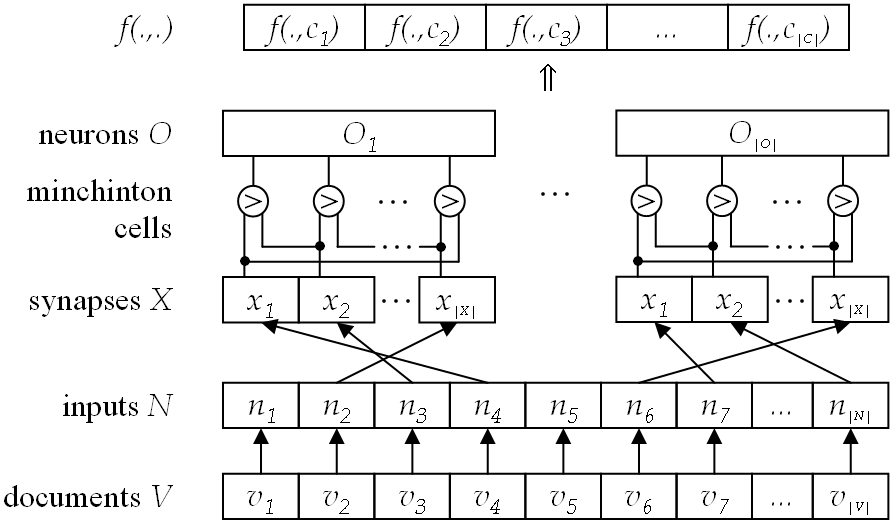
\includegraphics[width=0.6\textwidth]{imagens/arquitetura}
        \end{center}
    \end{figure}
\end{frame}
\subsection{Células de Minchinton}
\begin{frame}
    \frametitle{Células de Minchinton}
    \begin{itemize}
        \item pré-processamento
        \item dados de ``nível cinzento''
        \item três tipos:
            \begin{enumerate}
                \item limiar: $N[x] > constante$
                \item Tipo 0: $N[x1] > N[x2]$
                \item Tipo 1: $N[x1] - N[x1 + 1] > N[x2] - N[x2+1]$
            \end{enumerate}
        \item Tipo 0 considerado melhor
    \end{itemize}
\end{frame}
\subsection{Exemplo}
\begin{frame}
    \frametitle{Exemplo Multi-Categorias}
    \begin{table}
        \centering
        \begin{tabular}{|c|c|c|}
            \hline
            tabela      & valor & resultado\\
            \hline
            entrada 1   & 10010 & categoria 1\\
            \hline
            entrada 2   & 10111 & categoria 2\\
            \hline
            entrada 3   & 01000 & categoria 3\\
            \hline
                        & $\Uparrow$ & $\Downarrow$\\
            \hline
            input       & 10101 & categoria 2\\
            \hline
        \end{tabular}
    \end{table}
\end{frame}
\subsection{Referências}
\begin{frame}
    \frametitle{Referências}
    \tiny
    \begin{description}
        \item[Mult-Label Text Categorization Using VG-RAM Weightless Neural Networks] Badue, C., Pedroni F. and De Souza, A. F. \emph{In} 10th Brazilian Symposium on Neural Networks
        \item[Comparison of Some Methods for Processing 'Grey Level' Data in Weightless Networks] Mitchel, R. J., Bishop, J. M., Box, S. K. and Hawker, J. F. \emph{In} RAM Based Neural Networks - World Scientific
        \item[From WiSARD to MAGNUS: a Family of Weightless Virtual Neural Machines] Aleksander, I. \emph{In} RAM Based Neural Networks - World Scientific
        \item[A Brief Introduction to Weightless Neural Systems] Aleksander, I. De Gregorio, M., França, F. M. G., Lima, P. M. V., and Morton, H. \emph{In} ESANN'2009 proceedins, European Symposium on Artificial Neural Networks - Advances in Computational Intelligence and Learning
        \item[Weightless Neural Models: a Review of Current and Past Works] Ludermir, T. B., De Carvalho, A., Braga, A. P. and De Souto, M. C. P. \emph{In} Neural Computing Surveys 2
        \item[Multi-Label Text Categorization with a Data Correlated VG-RAM Weightless Neural Network] De Souza, A. F., Meloltti, B. Z. and Badue, C. \emph{In} Internation Journal of Computational Intelligence Research
    \end{description}
\end{frame}
\end{document}
